\documentclass[article]{report} % Type of document

\usepackage[utf8]{inputenc}    		 	% Encoding
\usepackage[english]{babel}			% Language
\usepackage{geometry}           			% Page margin
\usepackage{graphicx}           			% For images
\usepackage{newcent}            			% Font
\usepackage{color}              			% Colors
\usepackage{listings}           			% Lists
\usepackage[footnote, nolist]{acronym}	% Acronyms
\usepackage[absolute, overlay]{textpos}	% Text positioning

\usepackage{fancyhdr}          			 % We might have a need for them
\usepackage{float}
\usepackage{tabularx}

\usepackage{latexsym}
\usepackage{pdfpages}
\usepackage{tikz}
\usepackage{ifthen}
\usepackage{wrapfig}
\usepackage{textcomp}
\usepackage{multicol}

\setlength{\columnsep}{1cm}
\setlength{\TPHorizModule}{\paperwidth}	% Used for textblock
\setlength{\TPVertModule}{\paperheight}	% Used for textblock

\title {Oral Presentation 1}
\parskip = 0.25cm              % Summary options (spaces between lines)

% Margin
\geometry{tmargin=2.5cm, bmargin=1.5cm, lmargin=2.5cm, rmargin=2cm}

\definecolor{blue}{rgb}{0.13,0.29,0.46}
\definecolor{red}{rgb}{1,0,0}
\definecolor{couleur_titre}{rgb}{0.20, 0.45, 0.80}
\definecolor{couleur_nom}{rgb}{0.11, 0.6, 0.18}

\renewcommand{\labelitemi}{$\bullet$}
\renewcommand{\contentsname}{Table of contents}

% Title at the top of the page
\pagestyle{fancyplain} \chead{}\lhead{\textit{Team Dedalus}} \rhead{\textcolor{couleur_titre}{\emph{\textit{Project: SkyLands}}}}

\title {Book of specifications}
\author {Romain\and Renaud\and Aenora\and Erwan}
\date {}

%
% Document
%
\begin{acronym}
	\acro{OO}{Oriented-Object}
	\acro{RTS}{Real Time Strategy}
	\acro{FPS}{First Person Shooter}
	\acro{Mogre}{Managed Object-Oriented Graphics Rendering Engine}
	\acro{API}{Application Progamming Interface}
	\acro{GUI}{Graphical User Interface}
	\acro{MyGUI}{Multilayer and overlappable GUI System}
	\acro{IDE}{Integrated Developement Environment}
	\acro{AI}{Artificial Intelligence}
	\acro{NPC}{Non Player Character}
	\acro{UML}{Unified Modeling Language}
	\acro{PHP}{PHP : Hypertext Preprocessor}
	\acro{ORM}{Object-Relational Mapping}
	\acro{MVC}{Model View Controller}
	\acro{OGRE}{Object-Oriented Graphics Rendering Engine}
\end{acronym}
\begin{document}
		\thispagestyle{empty}
  			\begin{titlepage} 
						\vspace*{1cm} 
  					\begin{center} 
  							{\huge{\textsc{1st Oral} \\ ~ \\{\large From}\\ ~\\ Team \\  ~ \\ }}
	  						\includegraphics[width = 14cm]{images/Titles/Dedalus.png}
							\\ ~ \\ ~ \\ ~ \\ ~ \\ ~ \\ ~ \\ ~ \\ ~ \\ ~ \\ ~ \\ ~ \\ ~ \\ ~ \\ ~ 
						\end{center}
  					\hfill {\large Romain \textsc{Biessy}}
  					\hfill {\large Renaud \textsc{Gaubert}}
  					\hfill {\large Aenora \textsc{Tye}}
  					\hfill {\large Erwan  \textsc{Vasseure}}
  			\end{titlepage} 

  	\tableofcontents
  		\pagenumbering{arabic}
  		\newpage
		
		\chapter{\textcolor{blue}{Introduction}}
 			An ambitious 3d game such as ours requires a lot of work, to give you an example we spent not less than 100 hours each on the project since October also our project actually counts 120 000 characters and 15 000 lines of codes with not less than a 100 files.\\
			
			This game also required a constant load of work from ourselves : 
			\begin{figure}[h]
				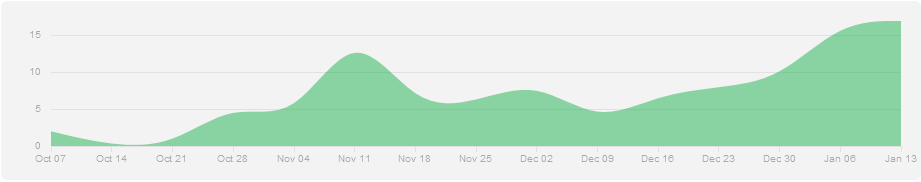
\includegraphics[width=18cm]{images/Schemas/stats.png}
			\end{figure}

 			Of course this would be meaningless if we wrote bad code, even if we don't have the pretension to say that we write good code we have the pretension to say that  we do note write bad code.

 			Throughout this report we will try highlight the fact that our work has payed and we already have a good base to proceed without worrying about the development of our game.


								
  		\chapter{\textcolor{blue}{Scripts}}
			\section{First script}
				As time went on, we thought of a better scenario than the one elaborated for the book of specifications. 
				And we came up with two scenarios of our own : \\

				During the second half of the XXIVth century war has been declared between the human race and the Kabool empire.The whole universe 					has become a large battlefield, not providing any safe shelter. As war goes on, the Kabool empire has finally taken over the Gaia systeme, 					your homeland and the very core of the universe. They plan to destroy the Genesia, a purelight gemstone that keeps the universe balance.\\

				 If the Genesia were to be destroyed, the whole system would blow appart and create a black hole that could end up swallowing 						everything. The gemstone is kept on a secret planet named Utopia, made from flying islands floating thanks to the mystic power of the 					Genesia.\\

 				As the threat over it grows larger, the islands are beginning to crash due to lack of the power from the Genesia being taken away. You embody a legendary soldier send to Utopia to retrieve the gemstone under the enemy eye and chase the Kabool empire away from the 					planet.\\

				You will have to conquer the planet, island after island by developing a colony with your soldiers and discover new technologies that allow 
				you to travel from one island to another and will help you win again the Kabool and save the universe.
				You finally land on the planet, and here your journey begin. 

\begin{center}				
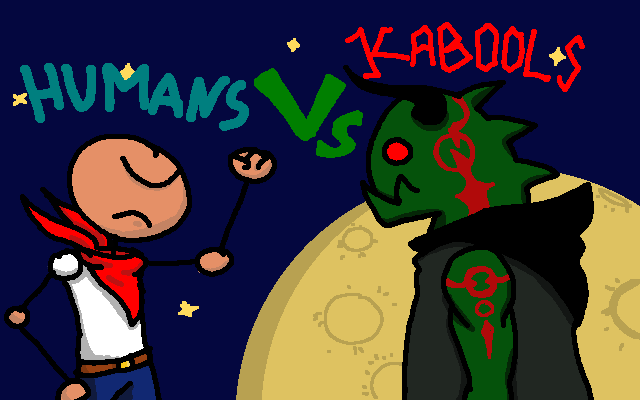
\includegraphics[width=10cm, height=5cm]{images/Others/fun.png}
\end{center}

				\newpage
			\section{Second scipt}
				\begin{figure}[h]
				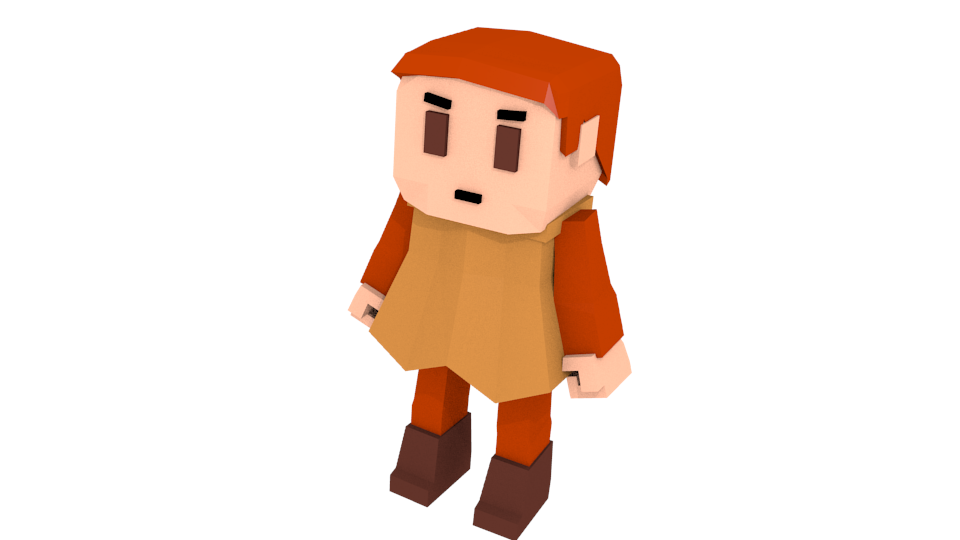
\includegraphics[scale=0.8]{images/Graphics/char.png}
				\end{figure}
				\begin{textblock}{0.22}(0.2, 0.21)
					 In the second part of the XXIVth century, the World Confederation, the galactical government faces a high amount of criminality from every planets of the federation.Some planets soon became populated by rebels and pirates.\\

 You are a miner from the planet Mangaria 2, sent to work into a mine on a crystal planet. The flight was supposed to last one year, but after 4 months and 15 days the alarms started to ring, a pirate ship started to attack you, you ship was lost, and you barely managed to escape with an escape pod. Your pod was programed to go to the nearest planet; the pirate planet.\\
				\end{textblock}


		\chapter{\textcolor{blue}{State management}}
			\section{What have been done}
				The state management system has been implemented by Romain. The idea is simple and efficient. There is an abstract class State which can basically be started up, updated and shutted down. Then two classes inherit State : MenuState and GameState with their own attributes. The most important class is the StateManager, it has a stack of State which can be easily popped and pushed from other classes using reflexion - we just have to specify the type of the state to the StateManager in order to push a state. Each frames, the StateManager updates only the first State of the stack so that the other States aren't destroyed but are liked paused since not updated.\\

This system has the advantage to structure the code. Besides, it makes the change from one State to another very easy.
			\section{What must be done}
		There isn't much work anymore for the state management. All we need now is to implement some other States such as an OptionState. Then it could be launched from any other existing State

		\chapter{\textcolor{blue}{Menu}}
			\section{What have been done}
				For now the menu is represented by three buttons, "Play", "Exit" and "Options". The play button will simply launch the terrain generation and after a few seconds put us into the character skin. The exit button does what you think it's doing. The options button does nothing for now. The background has been made into Minecraft since it's our graphic model; and our game is not fit enough for the task.
				\begin{center}
					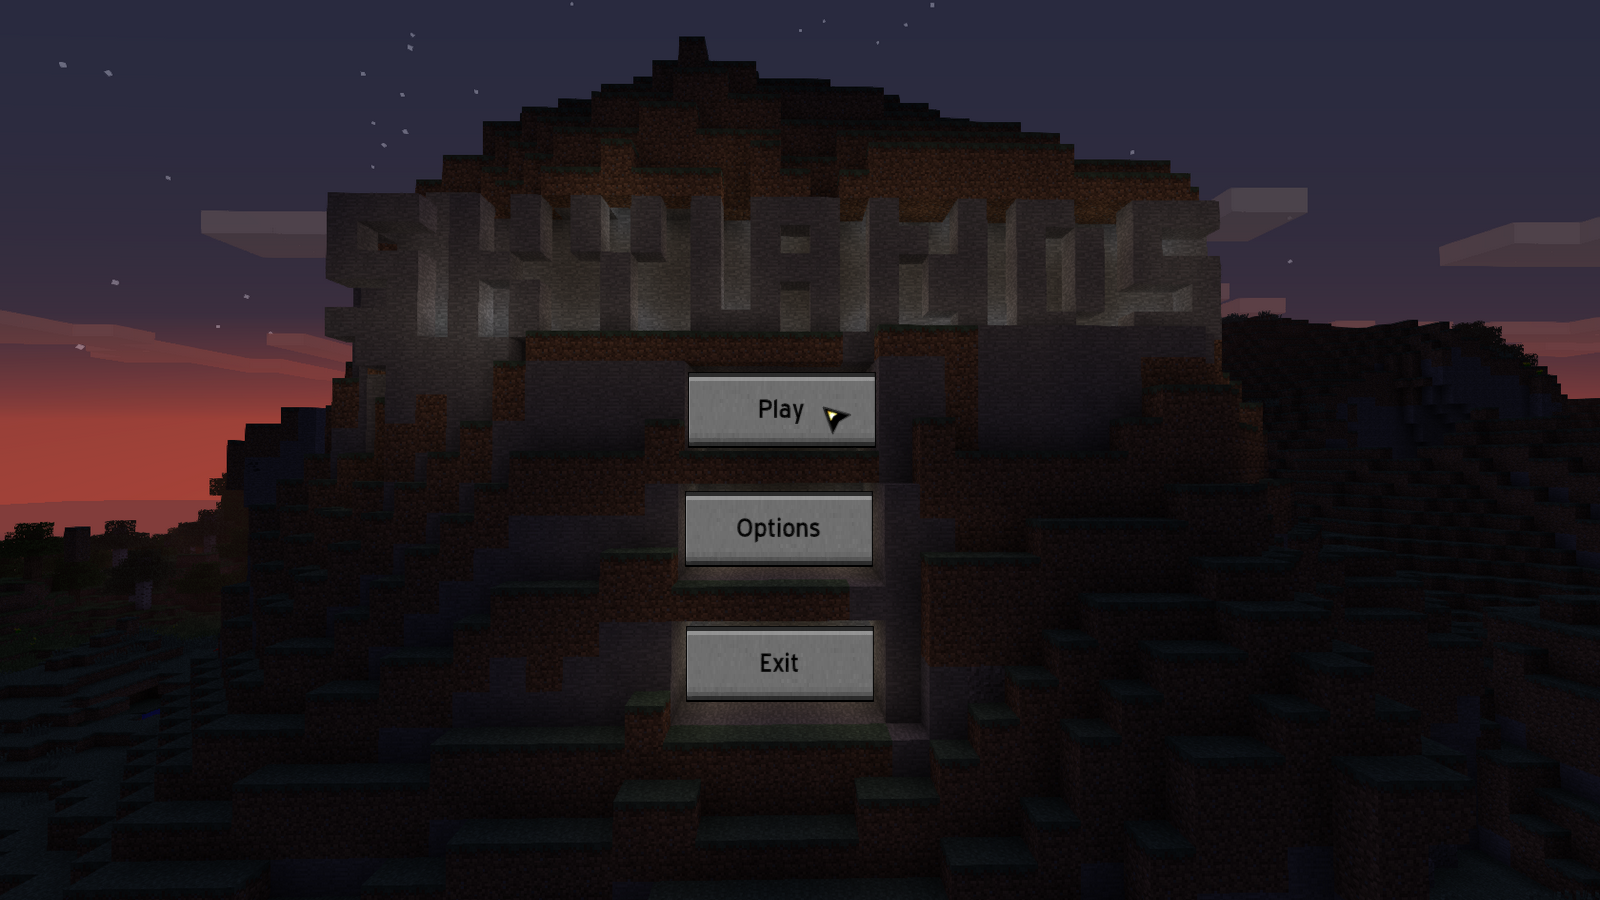
\includegraphics[width=17cm, height=10cm]{images/Screenshots/GameMenu.png}
				\end{center}
			\section{What's next}33
				Our goal for the next oral is to make a functional option button,  with few options like, the screen resolution, full-screen-windowed mode, the vertical sync, the language choice. We will also add an in-game menu.

		\chapter{\textcolor{blue}{Character}}
			\section{Mesh}
				At the beginning we were using the \ac{Mogre} mascot called Sinbad. It was useful since it has predefined animations; the drawback is that it doesn't have the right size, and it isn't made for being integrated in a cubic world. After that Aenora and Erwan made a few different characters in blender, a 3d software. We encountered difficulties while trying to implement the new mesh file and its animations into the \ac{Mogre} engine. Some of the character textures were made with the UV mapping technique.
				\begin{figure}[h]
					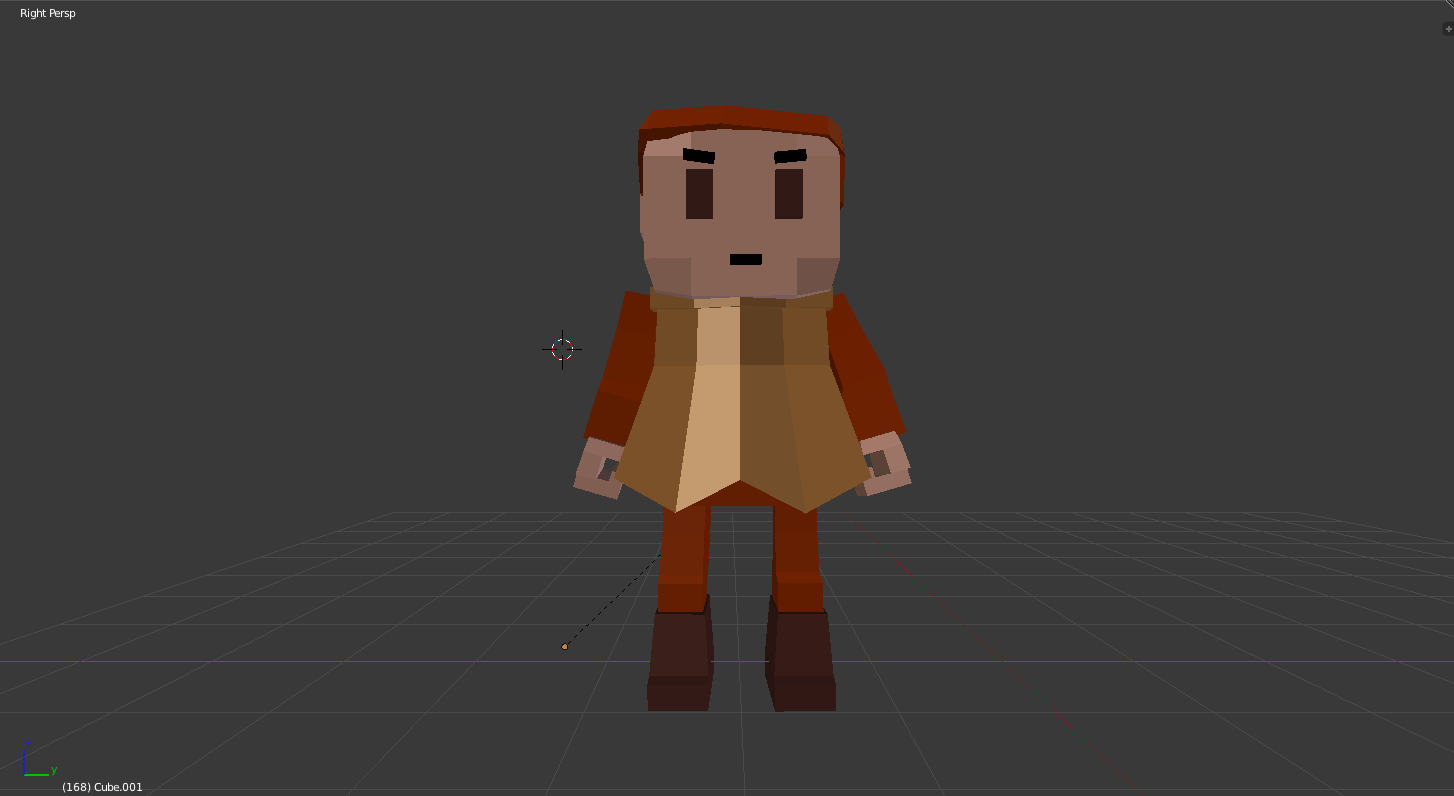
\includegraphics[width=8.5cm,   height=6cm]{images/Graphics/face_col.PNG}
					%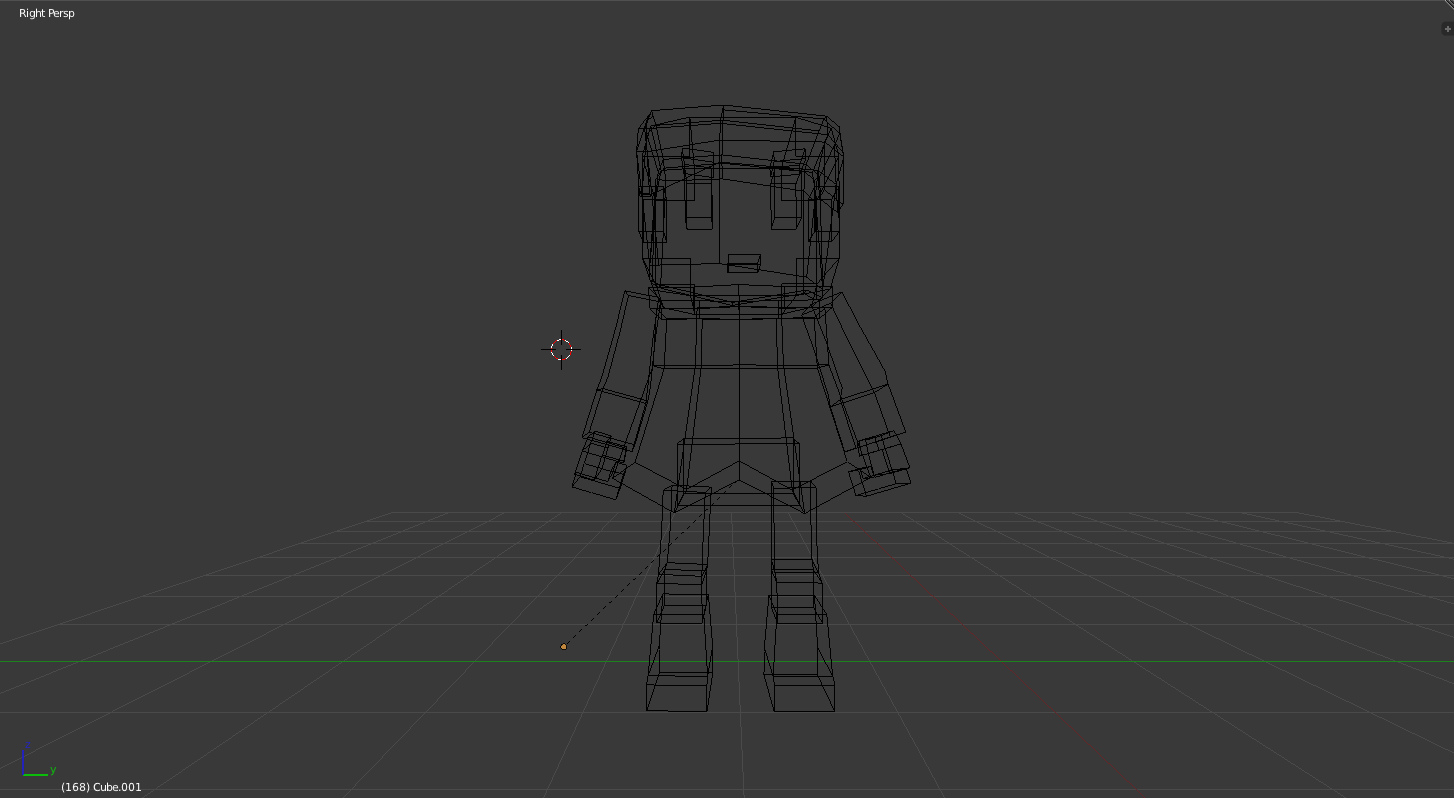
\includegraphics[width=8.5cm,   height=6cm]{images/Graphics/face_wire_col.PNG}
				\end{figure}
			\section{Move}
				We can move our character with the directional arrows or the WASD keys. Animations start by pressing one of these keys. There are four animations; two for the walking loop and two for the idle loop. Erwan integrated the keys manager, inspiring himself from the MOIS manager provided by \ac{Mogre}.\\

An issue Erwan encountered is the rotation of the player because we have a 3D world. If we needed some advanced rotations we would had to use quaternions, a powerful but non-intuitive mathematical tool similar to matrix in 4 dimensions. Fortunately an easier way is to decompose the rotation within the 3 axes (x, y, z). This is way simpler since we only need to rotations : yawing the player (around the y-axis) switch the horizontal movement of the mouse and pitching the camera (around the x-axis) switch the vertical movement of the mouse. Erwan implemented the rotation as well.
			\section{Animation}
				
				\begin{figure}[h]
				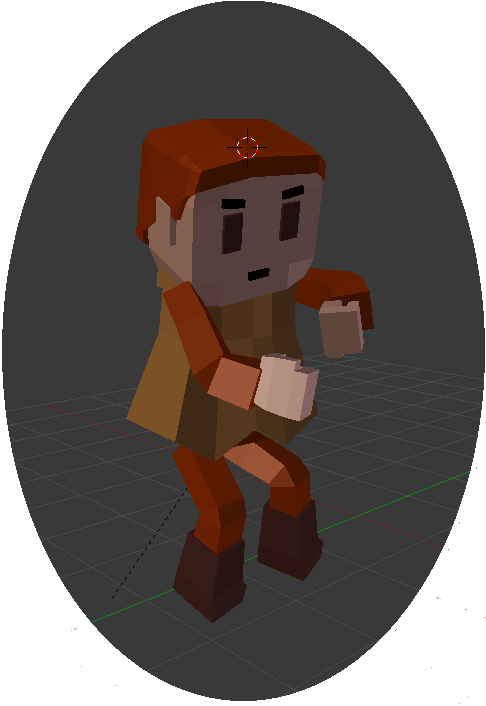
\includegraphics[width=6cm,   height=10cm]{images/Graphics/ex.png}
				\end{figure}
				\begin{textblock}{0.300}(0.5, 0.29)
					 Romain integrated a fade for the transitions of animation. Basically, animations have a weight between 0 and 1, 0 is no animation and 1 is the full animation, 0.5 would be that animation, but with a lower amplitude. The fade is made by decreasing the old animation's weight to 0, while increasing the new one to 1. This method guarantees a smooth transition between all the animations even if they are stopped before their end in game.
				\end{textblock}

			\section{Collision}
				The collision wasn't planed for this presentation but we have done the beginning. The hit-box of the character is represented by the 8 points of a parallelepiped rectangle. To test collision we look at the type of block around the character. For instance if we want to test the feet collisions, we get the type of the block under the character, using the 4 lowest points. For the next presentation, Romain will have to finish all the collisions test. The collision is still a little bit buggy and some work needs to be done. For sure, it will be fixed for the next presentation.

			\section{Camera}
				We can switch among two cameras in our game the first person one and the debug one. The first person camera is following the player, it just has to be pitch depending on the mouse. The debug camera isn't supposed to be seen by a player, thought it is very useful for us since it's a free camera detached from the player. Thus, we can see the whole world and the player with its animations. They have been both implemented by Romain.

			\section{What's next}
				Once the collision is fixed, we would like to implement the jump of the character. It's an essential feature that any \ac{FPS} game should have.
		\begin{figure}[h]

\includegraphics[scale=0.8]{images/Others/comingsoon.png}
\end{figure}
		\chapter{\textcolor{blue}{Graphic engine and terrain}}
			\section{Ogre3D}
				A 3D world is at first sight more complex than you could imagine.The player moves via an FPS (Fisrt Person Shooter) type camera. While its position in space is given by a Vector3 (3 floats). The orientation of the camera uses rotations around the X and Y axes: this is called respectively the yaw and pitch (the roll, rotation around the Z axis is not useful in our cases).
			\begin{figure}[h]
				
\includegraphics[width=11cm,   height=7cm]{images/Schemas/axis.png}
				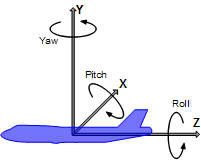
\includegraphics[width=6.5cm]{images/Schemas/Rotations.jpeg}
			\end{figure}
			
			A trick to find if the rotation you want to apply is a positive rotation or a negative rotation is the following : \\
			\begin{figure}[h]
				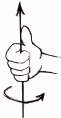
\includegraphics[]{images/Schemas/RotationsPositive.png}
			\end{figure}
			\begin{textblock}{0.628}(0.250, 0.825)
							\noindent  Using your right hand as a guide: point your thumb in the direction of an axis, curl your remaining fingers. The direction of the curl matches the positive rotation around that axis
			\end{textblock}
			\section{Terrain Generation}
				When creating the terrain architecture we had the goal to separate the terrain in multiple arrays which we called chunks. Thus, when we will be able to save the terrain, we won't save it in a single file. Also this permits us to later, dynamically load the terrain chunks by chunks and not as a single entity. \\
				The terrain Hierarchy is as follows : World contains a few islands which themselves contains a dictionary of chunks which contains a 16 * 16 * 16 array of blocks. It follows this chart : 
				\begin{figure}[h]
					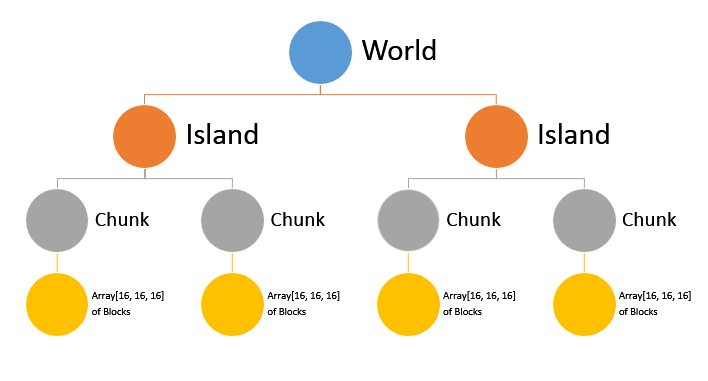
\includegraphics[width=18cm]{images/Schemas/WorldHierarchy.png}
				\end{figure}

				The terrain itself is generated when we create an island, using a fairly complex perlin 3d algorithm. \\
				The basic idea of the terrain generation is to go through all the blocks in each chunks of an Island, and with it's position,  using a 3D array of perlin noise, we compute the Block's noise value and following it's value we choose the block's type : air or grass.
\newpage

\begin{center}					
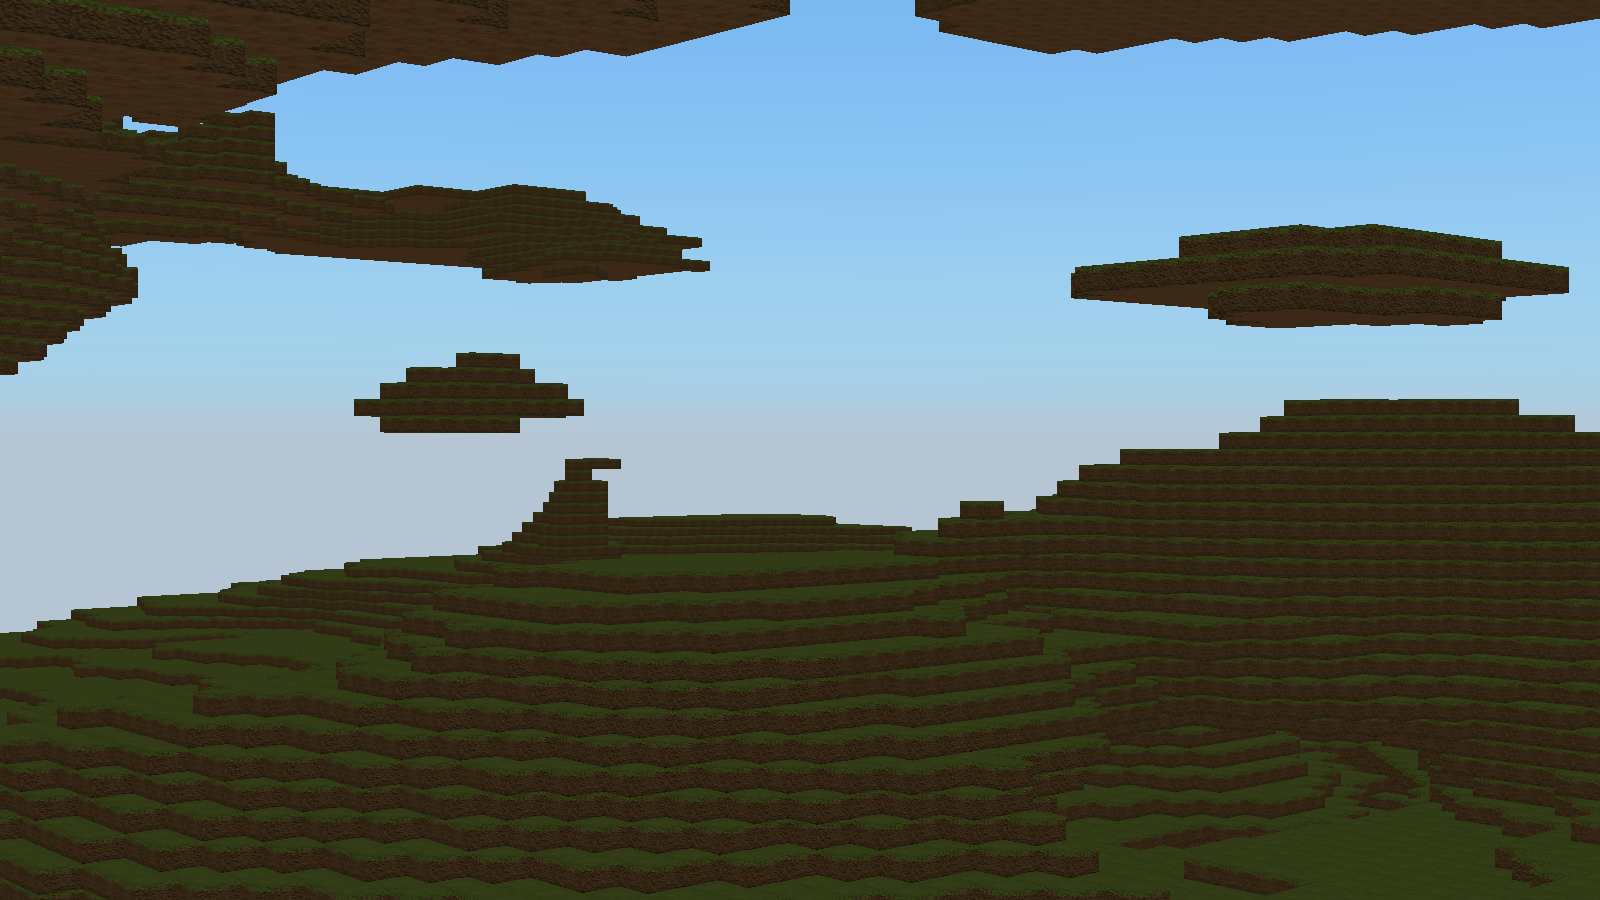
\includegraphics[width=16cm, height=10cm]{Images/Screenshots/Mountains02.png}
					\begin{center}\it A randomly mountain generated \end{center}
					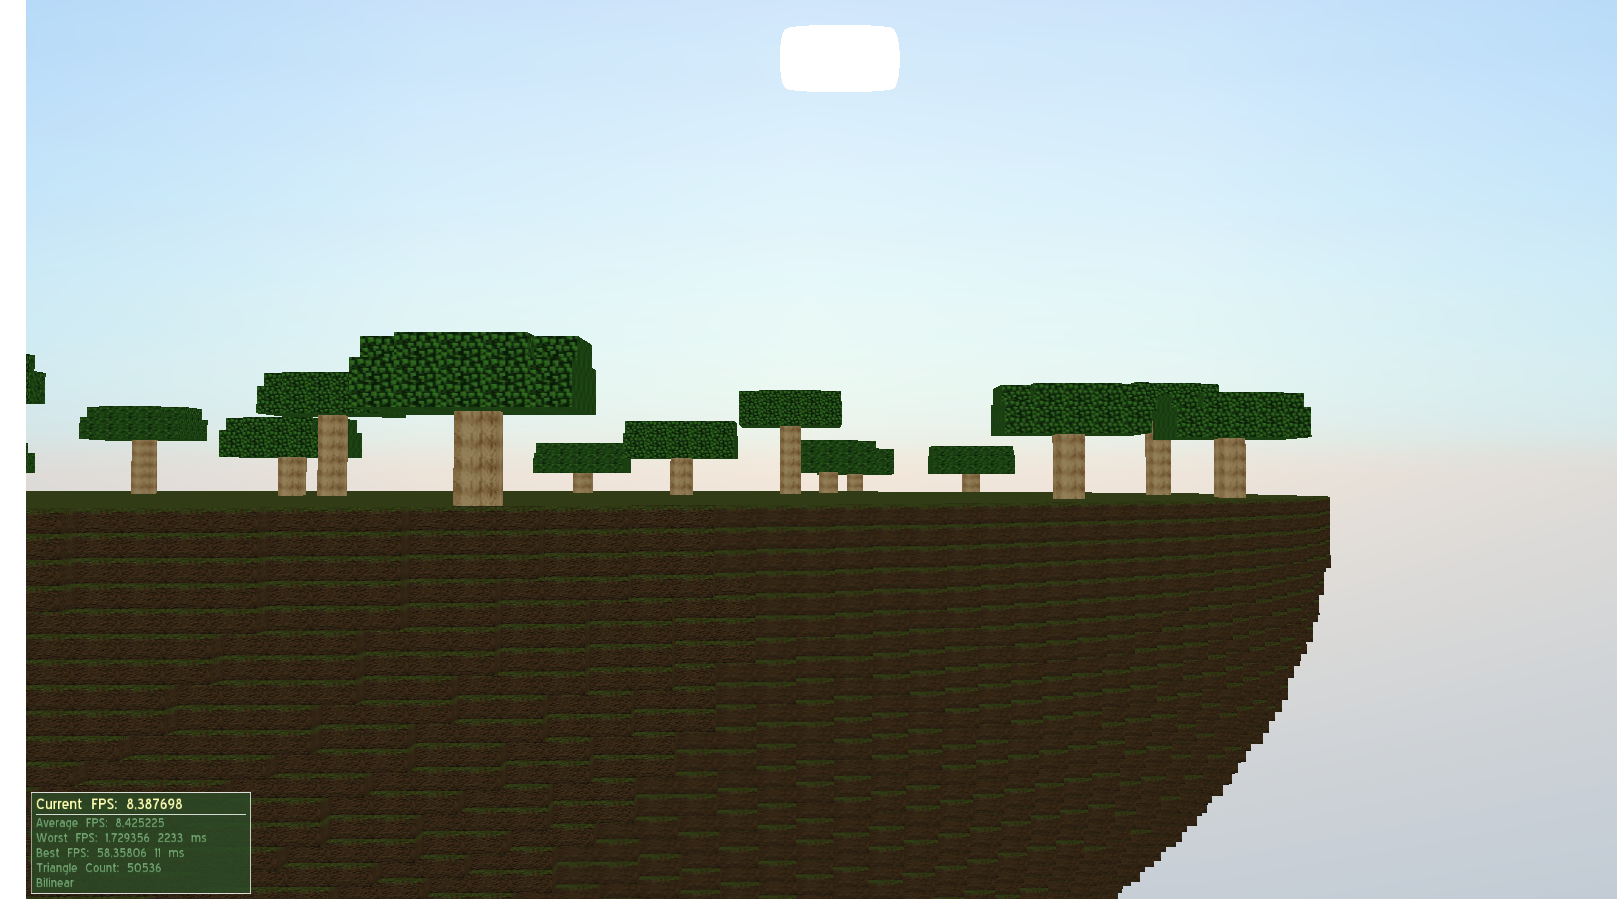
\includegraphics[width=16cm, height=10cm]{images/Screenshots/Dome02.png}
					\begin{center}\it A dome with random trees \end{center}
\end{center}

\newpage				
			\section{Terrain Display}
				Of course, displaying blocks where grass is, would've been to easy ! Indeed, even displaying visible blocks (to the player) cause a lot of lag, most of the time, with this method, the Frame Per Second count was below 1. \\
				
				Thus we had to imagine an other way to display blocks. The solution we have chosen is the following :
 				\begin{figure}[h]
					
\includegraphics[width=16cm, height = 8cm]{images/Schemas/ExplodedCube01.png}
					\begin{center}\it We exploded the cube into faces \end{center}
				\end{figure}
				\begin{textblock}{0.428}(0.450, 0.325)
					\noindent  We could have imported directly a cube from a mesh file. But we needed to have a specific texture for each faces. That's why we created the cube directly in our code face by face. The principal benefits are the fact that we can change the size of the faces from one variable.\\

 However, this still puts a large amount of entity on the screen, providing a number of FPS near 30. A good FPS count would be 60.
			\end{textblock}
			
			We exploded the block in 6 different faces. The basic idea is to create in the code the faces, copy them and assign them different textures : 
			\begin{figure}[h]
					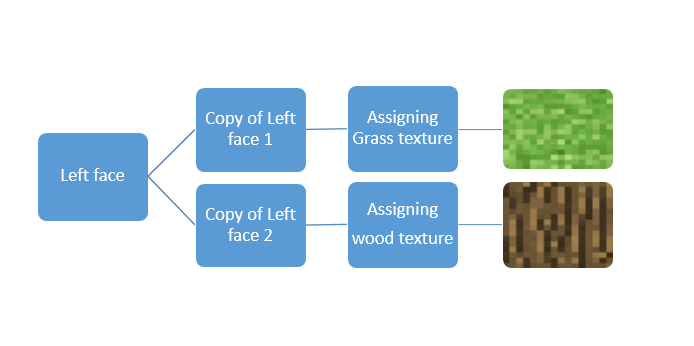
\includegraphics[scale=0.7]{images/Schemas/Display.png}
			\end{figure}
			\section{Sky}
				The sky is generated by an open source library : Caelum. The main difficulty was to build the lib ourselves related to the actual version of \ac{Mogre} we're using. It has been done by both Erwan and Romain. Then we just had to configure it.\\

			\begin{figure}[h]
				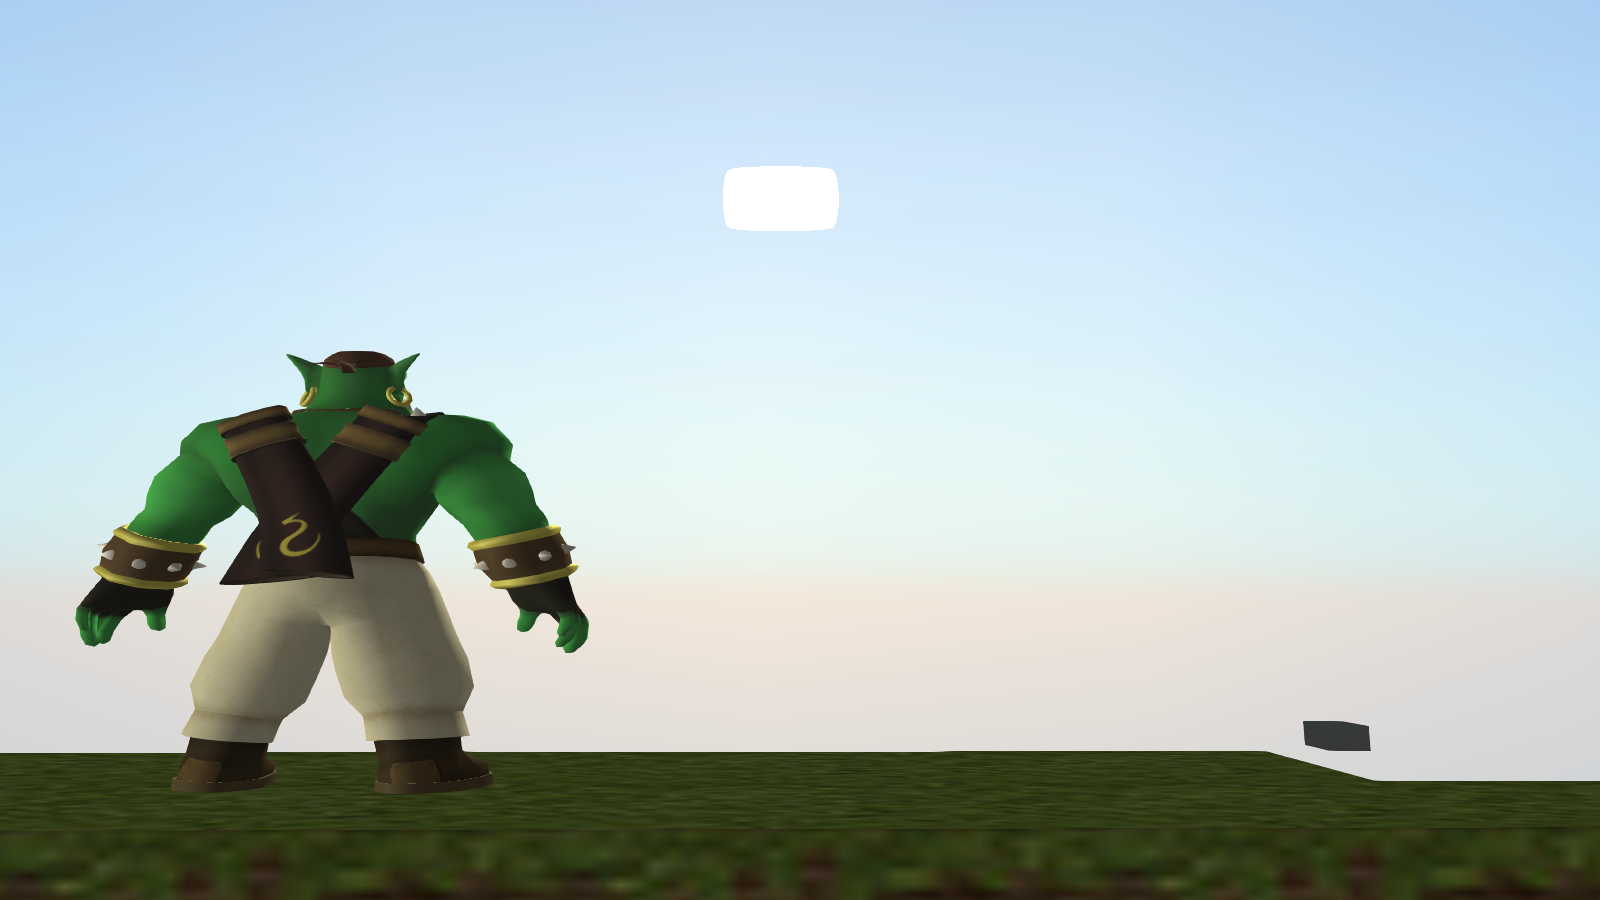
\includegraphics[width=15cm, height=8cm]{images/Screenshots/BackPerso-Sun.png}
\begin{center}\it \end{center}
				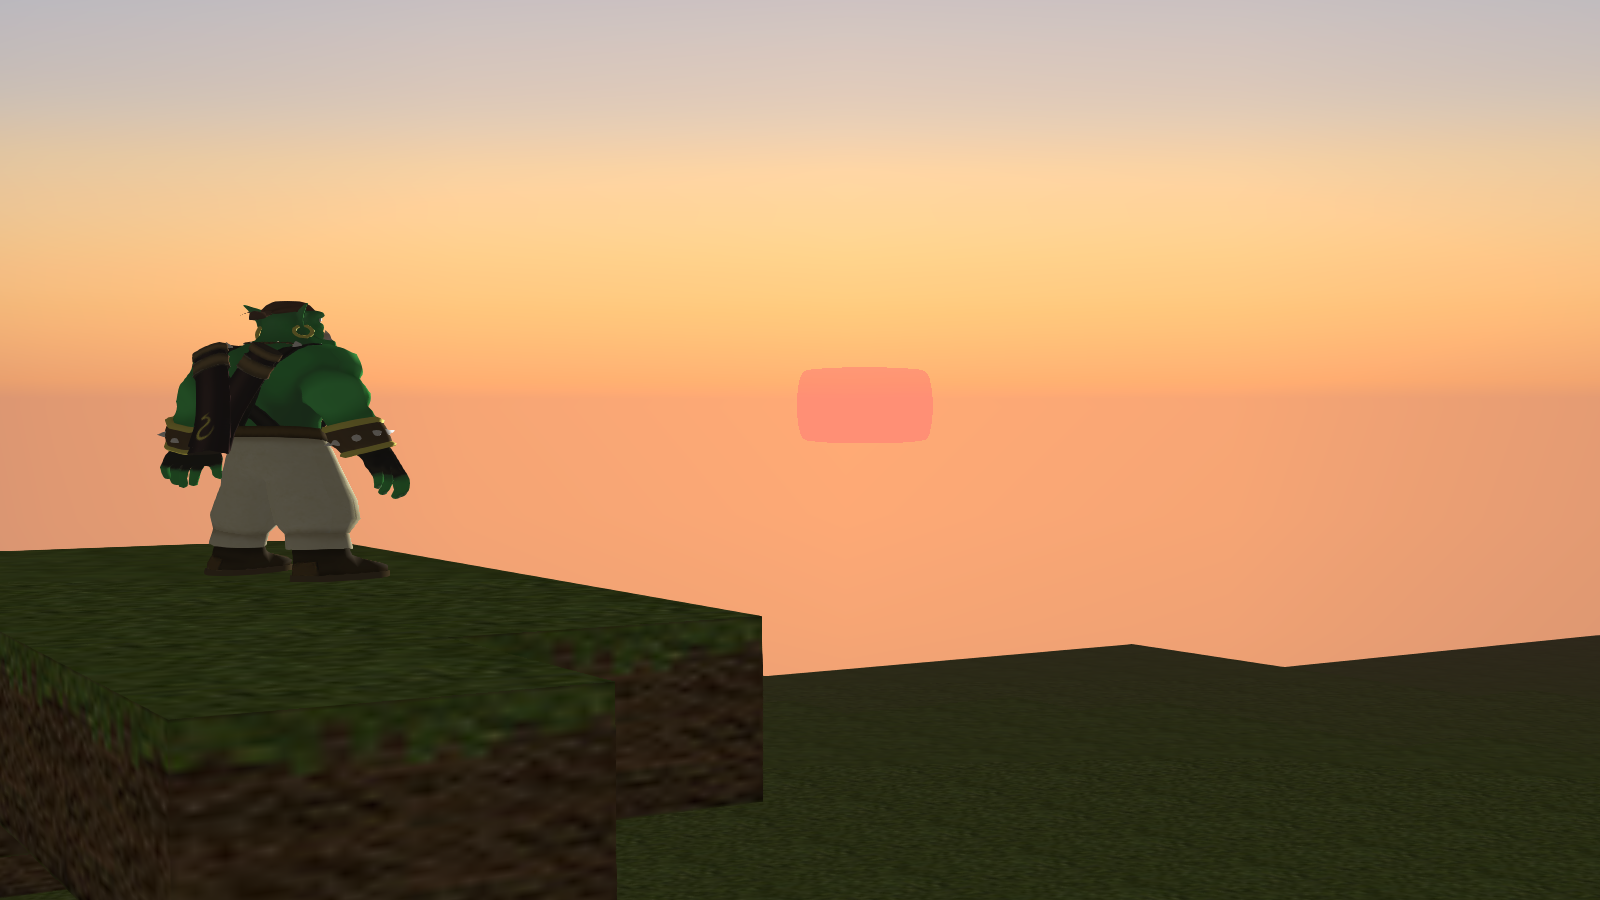
\includegraphics[width=15cm, height=8cm]{images/Screenshots/SunSet01.png}
				\begin{center}\it Dusk time on SkyLands. \end{center}
			\end{figure}
This lib is very useful, it automatically handle the position of the sun, the moon and the stars. Moreover it position the stellar objects according to the actual date and hour. We can easily speed up or down the time with the mouse wheel. Note that it won't modify the speed of the character.
\newpage
			\section{What's next}
				As we've already said, displaying faces has a major impact on the FPS count, thus the goal for the next oral presentation will be about having an other way of displaying the terrain (Vertex) or displaying not just faces but 'multi-blocks faces'. Either way, we need a better FPS count. \\

			Also you might have noticed that the terrain's borders seems to have been cut as if they were part of a bigger terrain. For the next oral we will have to cubically speaking round those borders. 

		\chapter{\textcolor{blue}{Graphics}}
			\section{Software choices}
 \subsection{Characters and 3D model:}
	To create the main character and enemies we used a 3D modeling software named Blender, that Erwan and Aenora already used in the past years.
Moreover, it is a free software and easy to use thanks to the large amount of on-line tutorials. Blender provides a broad spectrum of modeling, texturing, lighting, animation and video post-processing functionality in one package. Through its open architecture, Blender provides cross-platform interoperability, extensibility, an incredibly small footprint, and a tightly integrated work flow.
Despite being a free software, Blender provides the user an almost professional render. 
Edit mode lets you design the shape of your 3D model starting from a cube, a sphere or even a monkey head, then using UV editing mode, you can design texture for your shape using paint or photoshop or other similar programs.
\begin{center}
				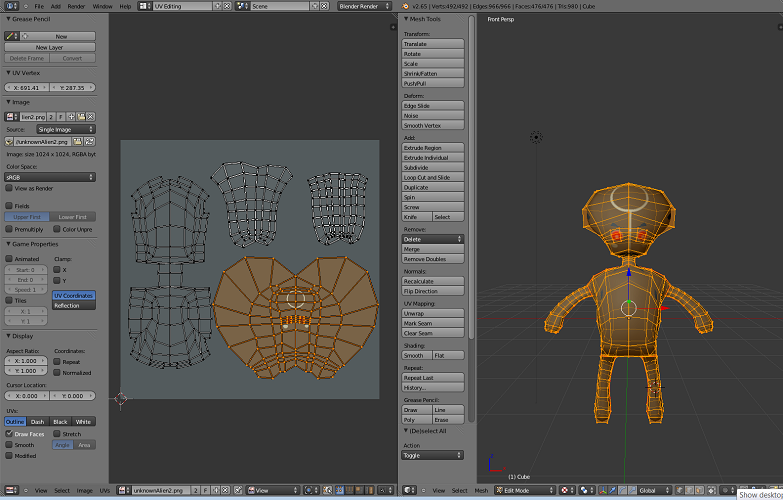
\includegraphics[width=14.5cm, height=9cm]{images/Graphics/UV_edit.png}
				\begin{center}\it You can place bones on your model to give it a structure and then animate it through the animation mode. 							\end{center}	
				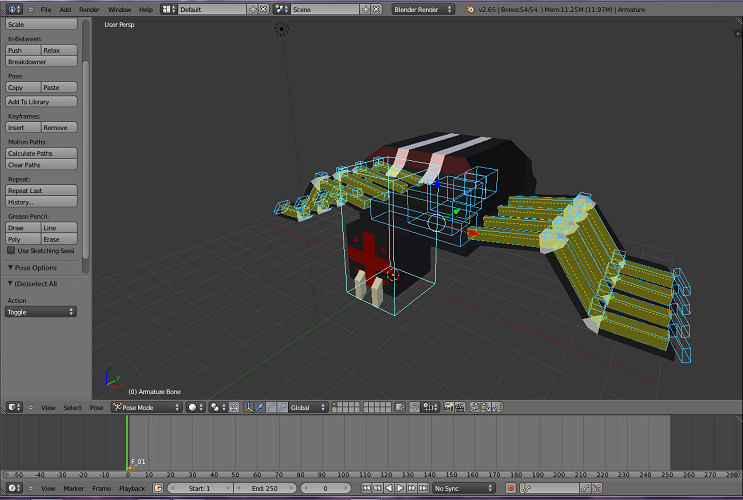
\includegraphics[width=15cm, height=8.5cm]{images/Graphics/spider_blend.png}
				\begin{center}\it Then link key-frames with the animations using the game engine. \end{center}
\end{center}
 \subsection{Texturing and illustrations:}
	As for the pictures and textures Aenora used photoshop since she already worked with it last year. The textures are 16x16 pixels images so that it takes the smallest place as possible. There are at least 20 different textures for all the different materials.\\

			%\begin{figure}[h]
				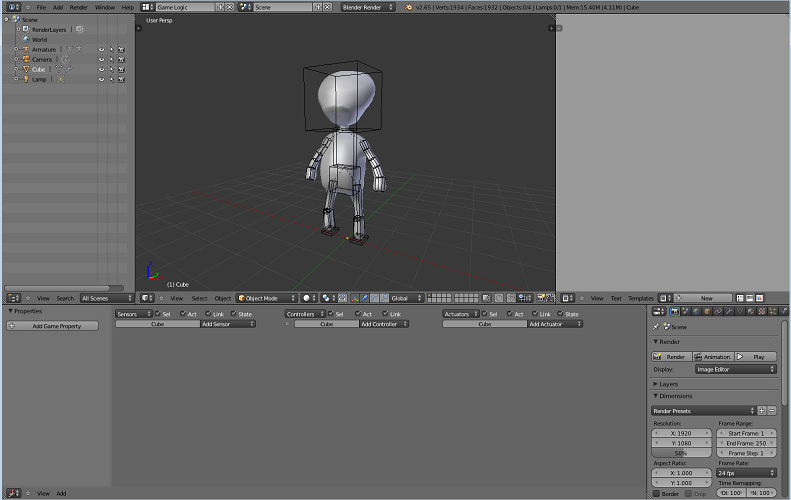
\includegraphics[width=15cm, height=9cm]{images/Graphics/game_engine.png}
				\begin{center}\it We finally fully created a player, enemies, weapons and 3D structures and animated them using blender. 							\end{center}
			%\end{figure}

\chapter{\textcolor{blue}{Website}}
				\section{PHP and JS}
					As explained in the book of specifications we are using the framework Symfony2. Which provides us a flexible OO interface. Of course symfony is not WordPress and we still have to work and code all the PHP but it provides useful components such as : easy URL rewriting, Templates, Form components, and automatic cache. \\
				\begin{figure}[h]
					
\includegraphics[scale=1.25]{images/Others/logo_symfony.png}
				\end{figure}
\\

As for the data storage Symfony2 uses Doctrine which uses a traditional SQL base and adds a database abstraction layer to the database. Thus with Doctrine, tables are class.\\

					As for the JavaScript, we used jQuery which is a fast and concise JavaScript Library that simplifies HTML document traversing, event handling, animation, and Ajax interactions. Thus, we could made animations in a few lines when using plain Javascript would've taken us hundreds of line.
\newpage
	
\begin{figure}[h]
					
\includegraphics[scale=1]{images/Others/jquery.png}
				\end{figure}

					Even thought we used a couple of library to simplify our work, keep in mind that they do not do the work for us, we still have to work with them to create the website.\\
 
				\section{Design}
					When creating our design, we wanted a maximum compatibility with the different browser (yes even IE 8 !), and even though the design isn't the same with a recent browser (such as Opera, Chrome, Firefox, Safari) than with an older browser which does not support CSS3, the deign does not appear ugly ! \\

					Using the new CSS3 properties and images created by our group members, we built our website by hand, during the winter holidays. As you might have guessed it was no easy task. Only one member of our group had done web coding before and was not a CSS expert.\\

					However, the result we came up with was surprisingly good looking : 
 
				\begin{figure}[h]
					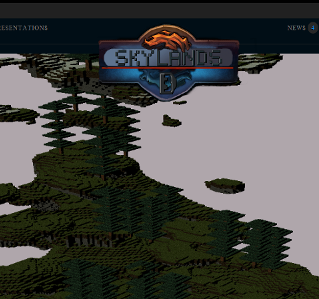
\includegraphics[scale=0.34]{images/Others/website.png}
				\end{figure}

		\chapter{\textcolor{blue}{Conclusion}}
			For this oral presentation, we've reached the goals we fixed in the book of specifications. Actually we did a bit more than we intended to do at first : Perlin 3d generation and Physics which required a lot of work !\\
			
			Our game's future seems bright, at the very beginning, when we thought the game,  we believed that our project might be a bit ambitious. However seeing our current progress in the game,  boosted up our moral and we are now convinced that we can finish this game !\\

			Still we better not lower our guard, the work we still have to do is enormous , and now that the base is done, we must not rest on our laurels.
	
				\begin{center}
					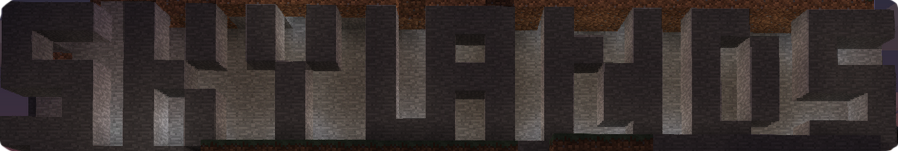
\includegraphics[width=16cm]{images/Titles/Skylands_logo.png}
				\end{center}     	     		
\end{document}